\section{Introduction}
\label{sec:intro}

Autonomous anomaly detection in multi-sensor telemetry monitors operational health across aerospace systems, Earth observation, cyber-physical infrastructure, and wearable digital healthcare \cite{meng2019spacecraft, chalapathy2019deep}. In remote sensing deployments (such as the NASA Soil Moisture Active Passive (SMAP) satellite, Mars Science Laboratory (MSL) rovers, industrial IoT facilities, and wearable biometric sensor arrays), dozens to hundreds of continuous telemetry channels concurrently track electrical power buses, thermal gradients, mechanical vibrations, and kinematics \cite{Hundman2018b}. When sensor faults or operational breakdowns emerge at the edge, monitoring systems must identify dynamical anomalies before hardware damage occurs \cite{cuellar2024explainable}.

\subsection{Challenges in Modeling Multi-Sensor Telemetry}
From a physical perspective, multi-sensor telemetry reflects the state trajectory of an underlying continuous physical system $\dot{x}(t) = \mathbf{f}(x(t))$. However, attempting to model dynamical equations directly in raw observation space presents four main challenges on edge devices:
\begin{enumerate}[leftmargin=*]
    \item \textit{Numerical Instability in Empirical Differentiation:} Estimating instantaneous time derivatives $\dot{x} \approx \frac{\Delta x}{\Delta t}$ directly on discrete, noise-corrupted sensor streams amplifies high-frequency measurement noise, destabilizing numerical trajectory tracking.
    \item \textit{Partial Observability \& Unmeasured Internal States:} Remote sensing telemetry captures only a noisy surface projection of unmeasured thermodynamic, electrical, and environmental states, violating full-state observability.
    \item \textit{High-Dimensional Cross-Sensor Coupling:} In multi-sensor IoT pods ($K \ge 50$), complex cross-channel dependencies and non-linear interactions cannot be adequately represented by rigid functional forms in raw signal space.
    \item \textit{Non-Stationary Downlink \& Operational Drift:} Edge IoT and satellite systems undergo discrete operational mode transitions (e.g., orbital day/night thermal cycling, thruster firings, Parkinsonian gait freezing, cloud server garbage collection) that cause continuous distribution drift.
\end{enumerate}

\subsection{Limitations of Deep Anomaly Detectors}
To bypass explicit equation modeling, deep learning architectures have emerged as data-driven alternatives, yet they remain constrained by three primary limitations:
\begin{enumerate}[leftmargin=*]
    \item \textit{Signal-Level Noise Memorization:} Traditional generative models (e.g., Autoencoders, VAEs, Masked Transformers) minimize point-level $L_1/L_2$ errors in raw signal space \cite{Hundman2018b, xu2022anomaly, wu2023timesnet}. Because reconstruction loss penalizes every point discrepancy equally, autoencoders expend substantial capacity memorizing high-frequency stochastic sensor jitter rather than learning the macro-scale dynamical laws governing nominal transitions.
    \item \textit{Limitations of Synthetic Contrastive Perturbations:} Contrastive frameworks like Neural Contextual Anomaly Detection (NCAD) \cite{carmona2021neural} train encoders via Contextual Outlier Exposure (COE) using heuristic synthetic perturbations (e.g., Gaussian noise spikes, sequence splicing). However, real physical faults manifest as subtle shifts away from nominal operating dynamics. Synthetic injections distort the learned embedding geometry, inducing artificial decision boundaries that produce false alarms on continuous physical streams.
    \item \textit{Conditional Mean Collapse in Multi-Branch Dynamics:} Deterministic predictive encoders trained with MSE loss $\mathbb{E}[\|\hat{z} - z\|^2]$ are mathematically constrained to predict the \textit{conditional mean} $\mathbb{E}[z_{\text{tgt}} \mid z_{\text{ctx}}]$. When physical systems possess multiple valid operational branches, the conditional mean lands in low-probability regions of representation space, triggering false alarms during legitimate multi-modal state transitions.
\end{enumerate}

\subsection{Our Approach: Dynamical Flow Matching for Edge Telemetry}
To address raw-space numerical noise and the reconstruction/collapse trade-offs of deep baselines, we evaluate a deterministic predictive baseline (Point-JEPA) and propose DyFlow-JEPA (Dynamical Flow-Matching Joint-Embedding Predictive Architecture). While flow matching has been explored in generative vision and robotics, we formulate flow matching for unsupervised anomaly detection in multi-sensor telemetry. Rather than integrating stiff trajectories in raw sensor space or reconstructing noisy waveforms, DyFlow-JEPA embeds the multi-sensor system into an abstract representation space and learns the continuous tangent velocity vector field of the nominal physical attractor manifold via Optimal Transport Conditional Flow Matching (OT-CFM) \cite{lipman2022flow}.

\begin{figure*}[t]
    \centering
    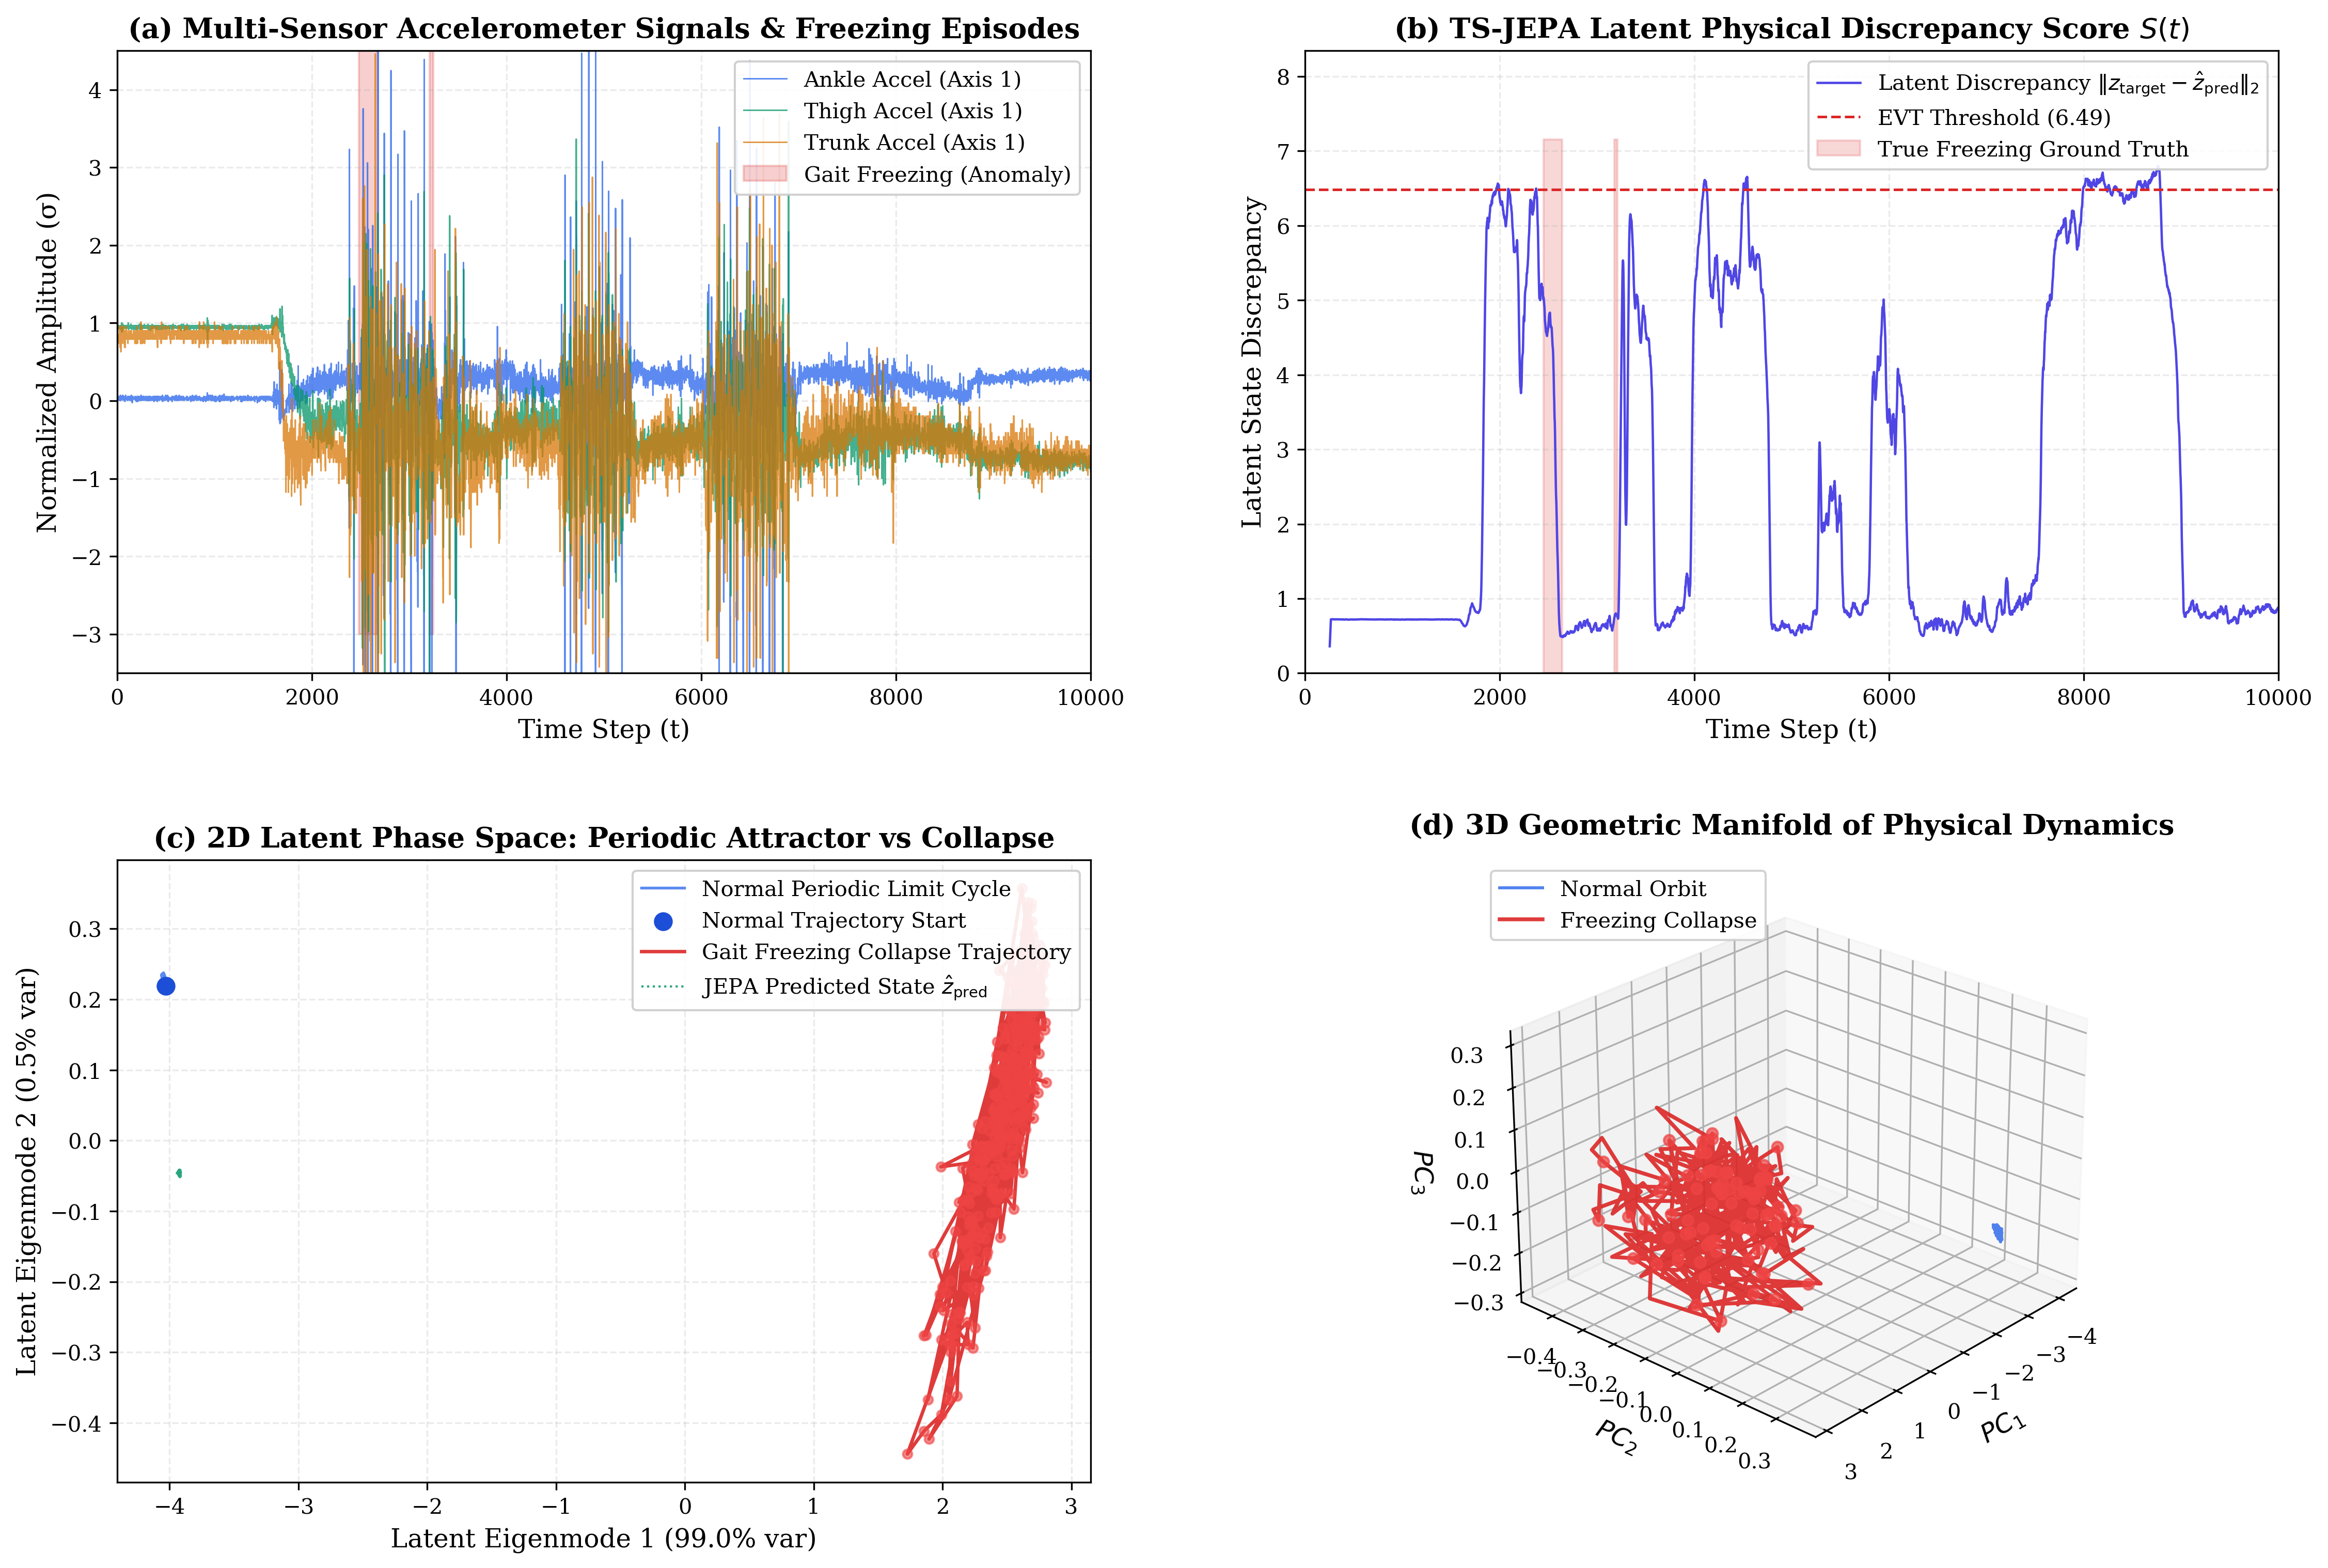
\includegraphics[width=0.95\linewidth]{figures/daphnet_phase_space_attractor.png}
    \caption{Phase-space dynamical analysis and anomaly detection with baseline Point-JEPA. (a) Raw multi-sensor accelerometry with ground-truth freezing-of-gait anomalies. (b) Point-JEPA latent discrepancy score $S(t) = \|z_{\text{tgt}} - \hat{z}_{\text{pred}}\|_2$ with EVT-calibrated decision threshold. (c) 2D and (d) 3D latent phase space: nominal dynamics form a stable periodic limit cycle (blue orbit), which the predictive encoder anticipates with near-zero error (green dashed line). When an anomaly occurs, the trajectory rapidly diverges from the attractor manifold (red line), generating a sharp, unambiguous anomaly signal.\label{fig:phase_space_attractor}}
\end{figure*}


As illustrated in Figure~\ref{fig:phase_space_attractor}, Point-JEPA maps nominal system behavior into stable limit-cycle attractors in representation space. In DyFlow-JEPA, a causal dilated Temporal Convolutional Network (TCN) or Patch Transformer context encoder processes historical context $x_{\text{ctx}}$, while a continuous flow velocity network $v_\psi(z_t, t, z_{\text{ctx}})$ models the probability paths leading to target representations $z_{\text{tgt}}$. The representation space is regularized via non-contrastive VICReg (Invariance, Variance hinge, Covariance decorrelation) \cite{bardes2021vicreg} to prevent dimensional collapse.

During inference on edge hardware, anomalous telemetry is detected by measuring the Deterministic Midpoint Velocity Discrepancy at $t=0.5$, whitened by an empirical Mahalanobis precision tensor $\mathbf{\Sigma}^{-1}$. Finally, Extreme Value Theory (EVT / SPOT) tail calibration \cite{siffer2017anomaly} establishes a decision threshold under the Pickands-Balkema-de Haan theorem, eliminating heuristic threshold tuning.

\subsection{Key Contributions}
The primary contributions of this work are as follows:
\begin{itemize}[leftmargin=*]
    \item \textit{Continuous Dynamical Flow Matching for Multi-Sensor Telemetry:} We formulate a continuous flow-matching joint-embedding framework for unsupervised anomaly detection in multi-sensor telemetry, modeling fault detection as continuous tangent velocity field learning on latent dynamical manifolds and avoiding conditional-mean collapse on multi-branching physical systems.
    \item \textit{Physical Attractor Geometry \& Non-Contrastive Regularization:} We formulate Optimal Transport Conditional Flow Matching within an EMA-regularized latent space, constrained by variance hinge and spectral covariance penalties to preserve dimensional rank across coupled sensor arrays without synthetic outlier injection.
    \item \textit{Deterministic Midpoint Evaluation \& Statistical Calibration:} We derive a zero-variance, single-pass deterministic midpoint velocity discrepancy metric ($t=0.5$) with second-order Taylor error bounds, coupled with Mahalanobis covariance whitening and Generalized Pareto Distribution (EVT / SPOT) extreme value calibration to set threshold-free decision alarms under low edge inference latency ($3.47$s).
    \item \textit{Multi-Sensor Telemetry Benchmark Evaluation:} Evaluated across 11 telemetry benchmark datasets comprising 130 continuous channels spanning four domain families (satellite remote sensing, wearable IoT, industrial testbeds, and smart infrastructure), DyFlow-JEPA outperforms deep baselines (TimesNet, TranAD, Anomaly Transformer, DCdetector, NCAD) under both channel-weighted and unweighted dataset macro metrics.
\end{itemize}



The remainder of this paper is structured as follows. Section~\ref{sec:related} reviews related work across equation discovery, reconstruction, contrastive learning, and JEPAs. Section~\ref{sec:dataset} describes the multi-sensor IoT and remote sensing benchmark suite. Section~\ref{sec:proposed_method} details the DyFlow-JEPA architecture, Optimal Transport flow matching, manifold regularization, and Mahalanobis EVT scoring. Section~\ref{sec:exp} presents the experimental setup, baselines, and grand benchmark evaluation. Section~\ref{sec:ablations} provides systematic ablation studies on loss formulations, latent capacity, and velocity discrepancy. Section~\ref{sec:results} discusses domain-by-domain insights, point-adjustment dynamics, and phase-space attractors. Finally, Section~\ref{sec:conclusion} concludes the paper and outlines future directions.

